\section{Typography}

%--------------------------------------------------------------------
%--- What is it about
%--------------------------------------------------------------------

\begin{frame}
\frametitle{What Is Typography About?}
Your final year project will consist of several elements:
\begin{itemize}
\item<2->
The mathematical content and the work you have done.
\item<3->
The words and sentences you use to describe the work.
\item<4-|alert@5-|trans:alert@1|handout:alert@1>
The way words and graphs are presented on the page.
\end{itemize}

\onslide<6->
\begin{center}
\begin{minipage}{0.8\linewidth}
\begin{block}{}
\textbf{typography} \emph{n}. The art and technique of arranging type to make written language legible, readable, and appealing when displayed.
\hfill\textsmaller{(Wikipedia)}
\end{block}
\end{minipage}
\end{center}
\end{frame}

\begin{frame}
\frametitle{Why Does Typography Matter?}
\begin{cvarblock}[0.9\linewidth]{}
%\textlarger

\hfill (Matthew Butterick, \emph{Typography for Lawyers})
\end{cvarblock}
\end{frame}

%--------------------------------------------------------------------
%--- Bold and Italic
%--------------------------------------------------------------------

\begin{frame}
\frametitle{\textbf{Bold} and \textit{Italic} Text}

\begin{columns}
\begin{column}{.46\linewidth}
\begin{block}<2,4>{}
\textlarger{%
\rmfamily
Within a larger body of text, a piece in \textit{italics} does not stand out much; instead it signifies a context difference only \textit{while} the text is being read. By contrast, a single word in \textit{boldface} attracts the human eyeball and is therefore recommended for keywords the reader might be \textit{looking} for.
}
\end{block}
\end{column}

\begin{column}{.46\linewidth}
\begin{block}<3,4>{}
\textlarger{%
\rmfamily
Within a larger body of text, a piece in \textbf{italics} does not stand out much; instead it signifies a context difference only \textbf{while} the text is being read. By contrast, a single word in \textbf{boldface} attracts the human eyeball and is therefore recommended for keywords the reader might be \textbf{looking} for.
}
\end{block}
\end{column}
\end{columns}
\end{frame}

%--------------------------------------------------------------------
%--- Bold/italic example
%--------------------------------------------------------------------

\begin{frame}
\frametitle{Bold and Italic in Use}
\begin{columns}[b]
\begin{column}{0.7\textwidth}
\fbox{%
\adjustbox{trim={0.8cm} {10.9cm} {5.4cm} {3.5cm}, clip, scale=0.7}{%
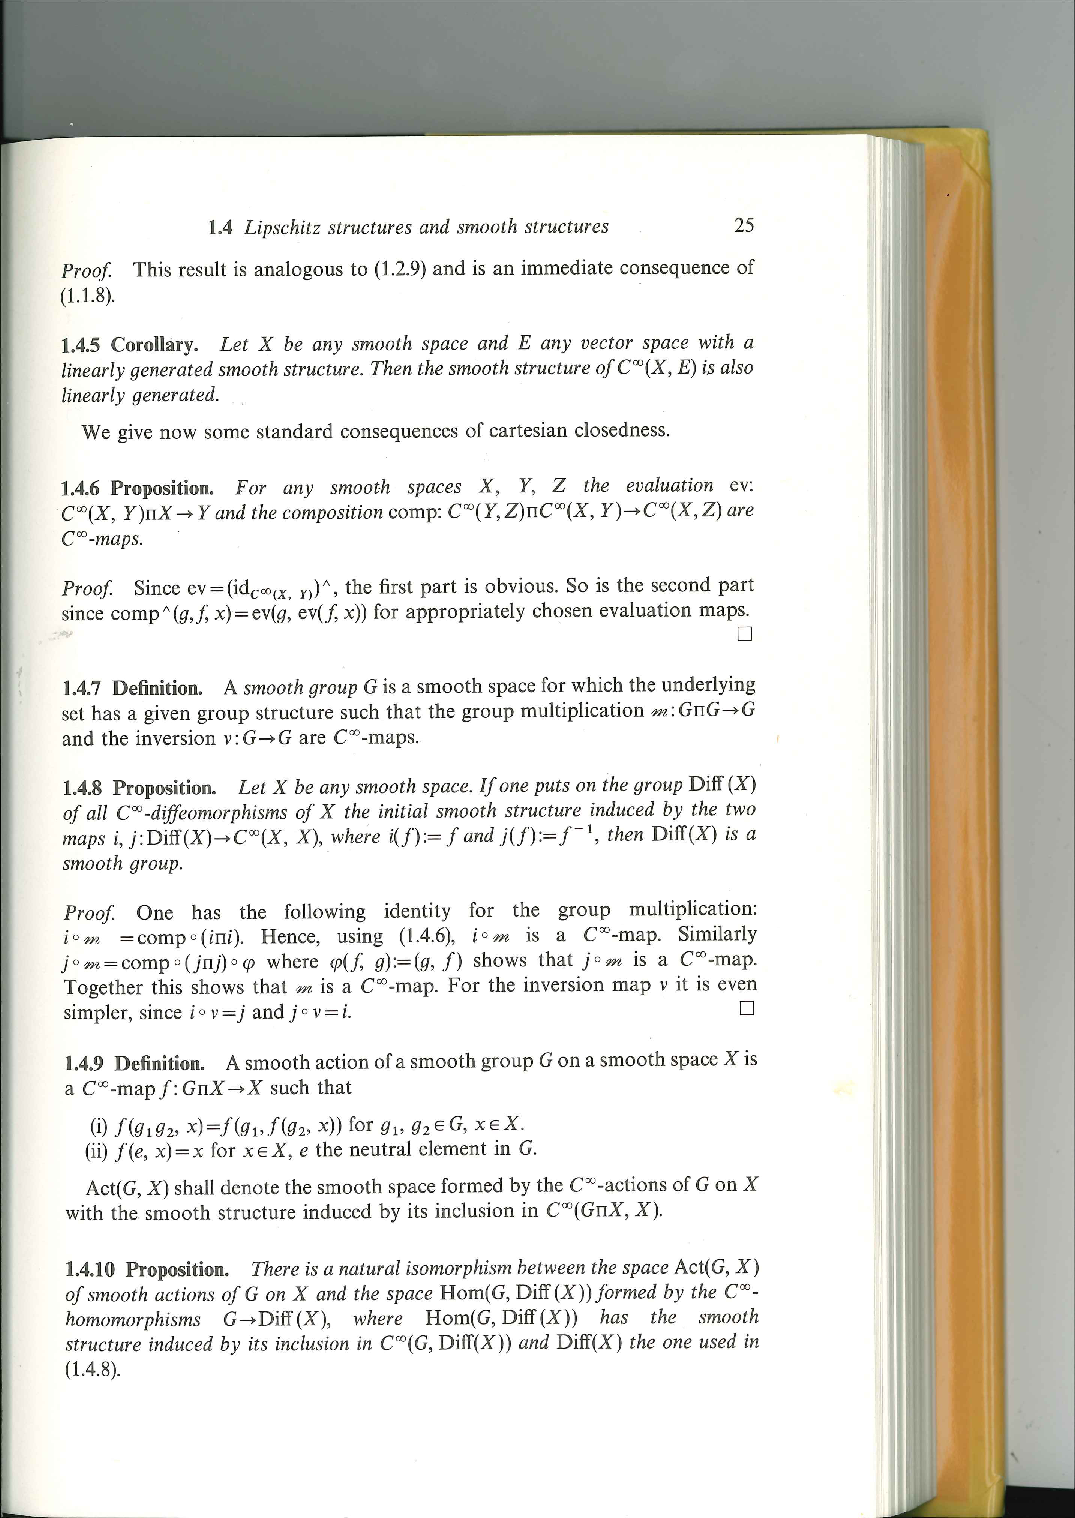
\includegraphics[width=182mm]{images/frolicher_kriegl_p25}}
}
\end{column}
\begin{column}{0.28\textwidth}
\textsmaller{
Alfred Fr\"olicher, Andreas Kriegl. \emph{Linear Spaces and Differentiation Theory}. John Wiley \& Sons. 1988.}
\end{column}
\end{columns}
\end{frame}

%--------------------------------------------------------------------
%--- Multiple columns
%--------------------------------------------------------------------

\begin{frame}
\frametitle{Multiple Columns}
\begin{center}
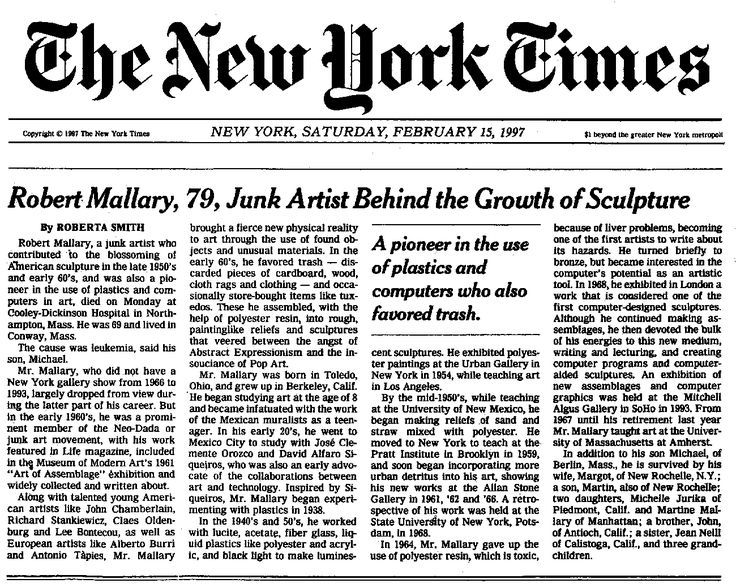
\includegraphics[width=0.83\linewidth]{images/nytimes_cover}
\end{center}
\end{frame}

%--------------------------------------------------------------------
%--- Page margins
%--------------------------------------------------------------------

\begin{frame}
\frametitle{Page Margins}
\begin{columns}
\begin{column}{0.5\textwidth}
\onslide<1->
\begin{center}
\vspace{-2em}
LibreOffice \medskip

\fbox{%
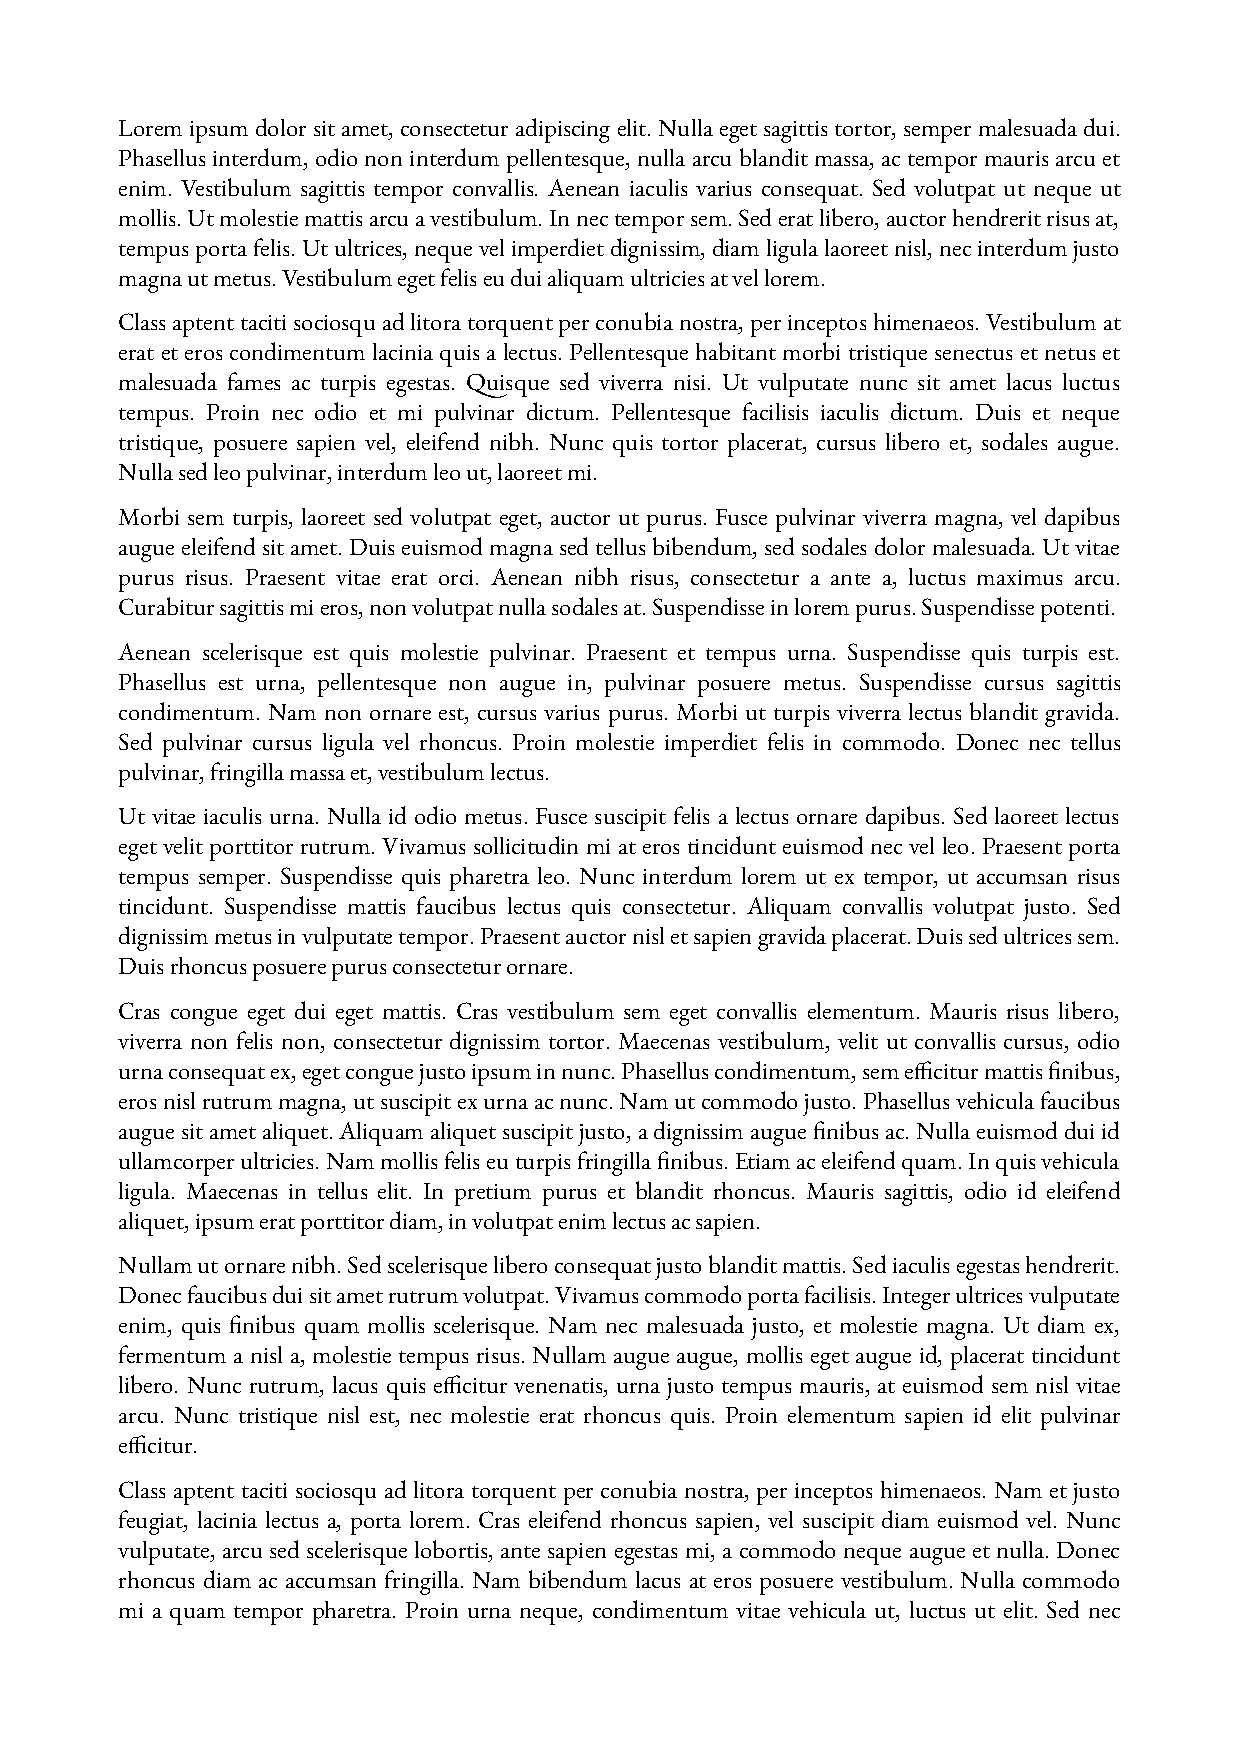
\includegraphics[width=.7\linewidth]{examples/word_lorem}
}
\end{center}

\onslide<2->
\textsmaller{Margins: L 2cm, R 2cm, T 2cm, B 2cm \\
Characters/line: 103}
\end{column}

\begin{column}{0.5\textwidth}
\onslide<1->
\begin{center}
\vspace{-2em}
\LaTeX\ article class \medskip

\fbox{%
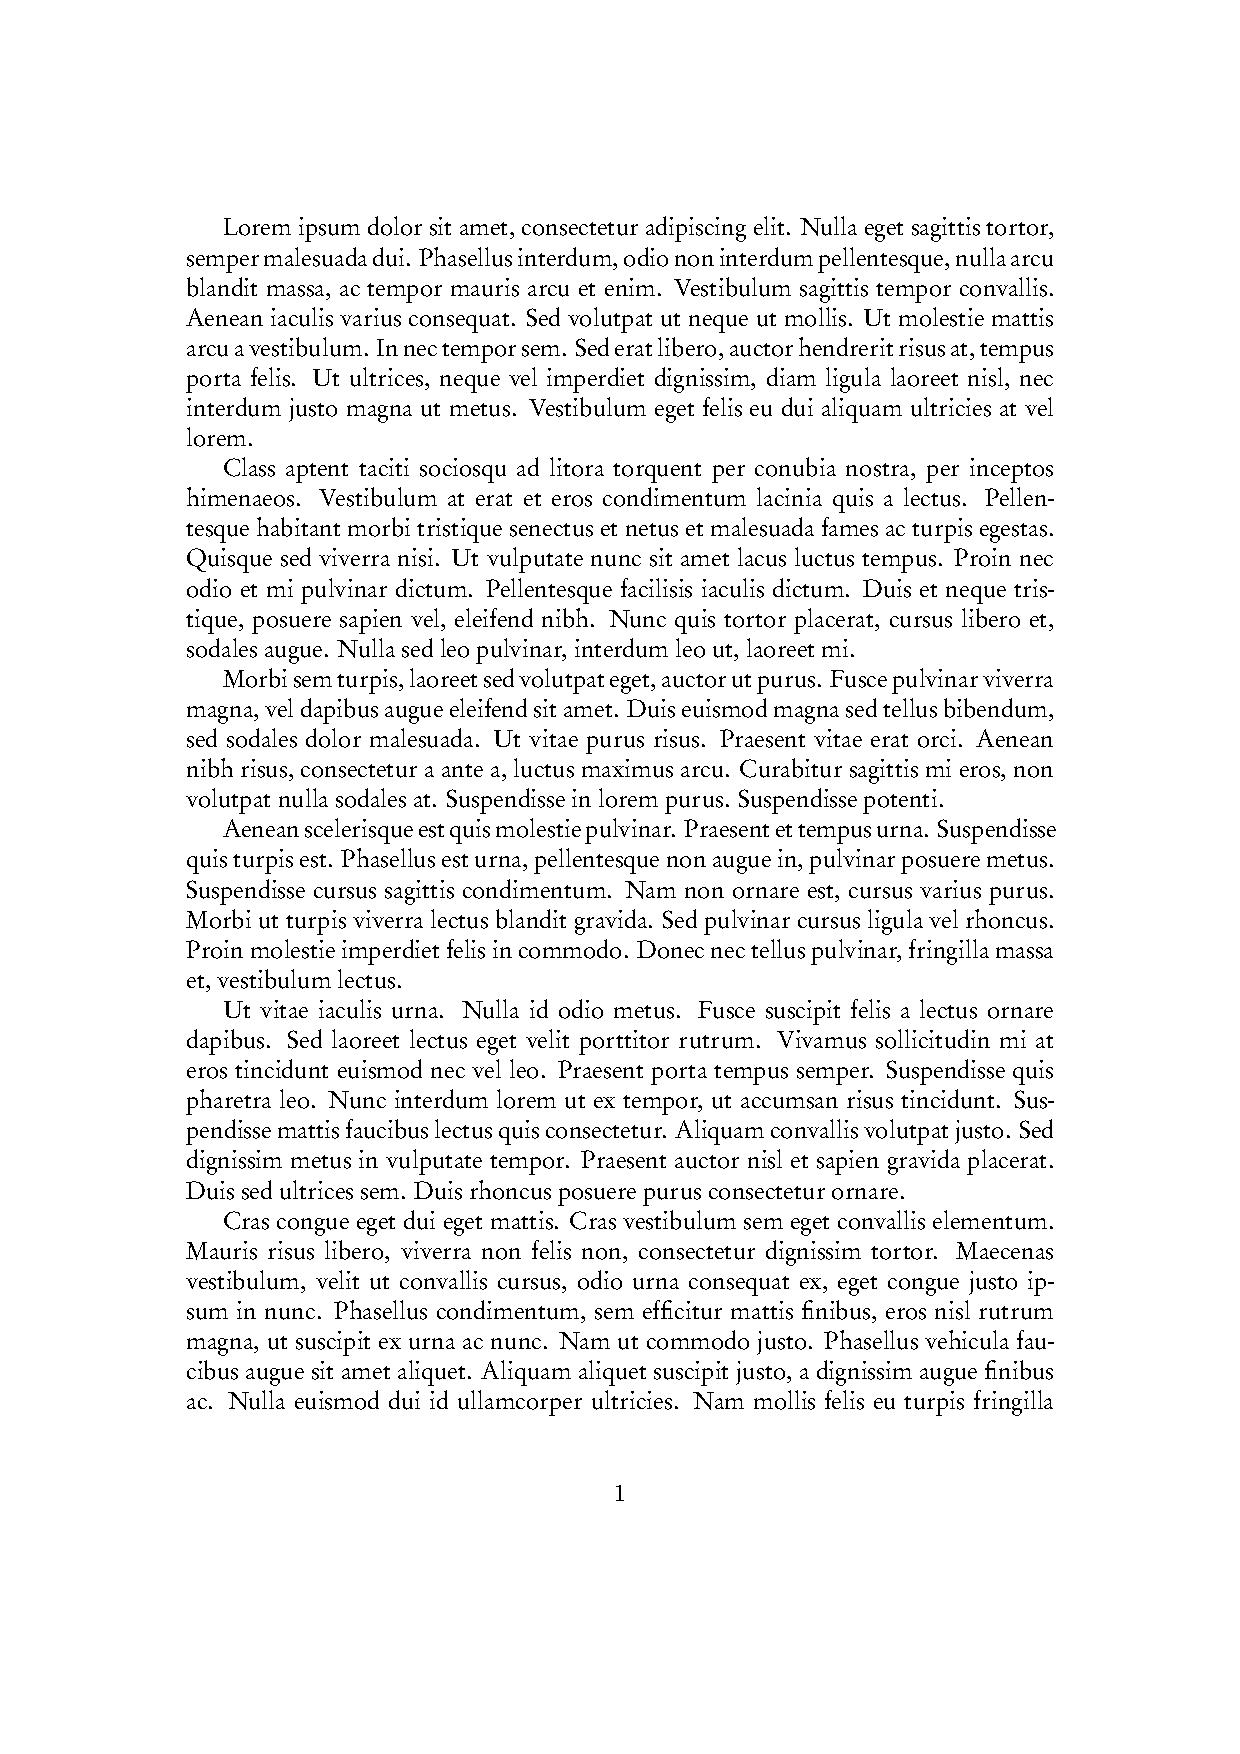
\includegraphics[width=.7\linewidth]{examples/latex_lorem}
}
\end{center}

\onslide<2->
\textsmaller{Margins: L 3cm, R 3cm, T 3.5cm, B 5.5cm \\
Characters/line: 85
}
\end{column}
\end{columns}
\end{frame}

%--------------------------------------------------------------------
%--- Book of Kells
%--------------------------------------------------------------------

\begin{frame}
\frametitle{The Book of Kells}
\begin{center}
\vspace{-1em}
\fbox{%
\adjustbox{trim={0px} {170px} {0px} {0px}, clip, scale=0.5}{%
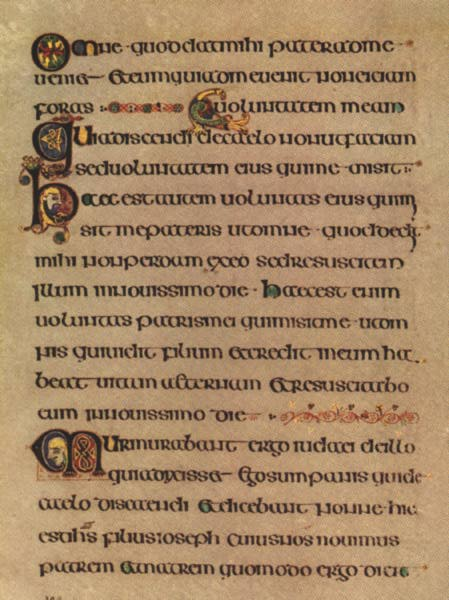
\includegraphics[width=449px]{images/book_of_kells}}
}
\end{center}
\vspace{-1em}
\hfill\footnotesize{Source: Wikimedia Commons
\href{https://commons.wikimedia.org/wiki/File:KellsFol309r.jpg}{(link)}.}
\end{frame}

%--------------------------------------------------------------------
%--- Gutenberg bible
%--------------------------------------------------------------------

\begin{frame}
\frametitle{The Gutenberg Bible}
\begin{center}
\vspace{-1em}
\fbox{%
\adjustbox{trim={0cm} {700px} {10px} {34px}, clip, scale=0.32}{%
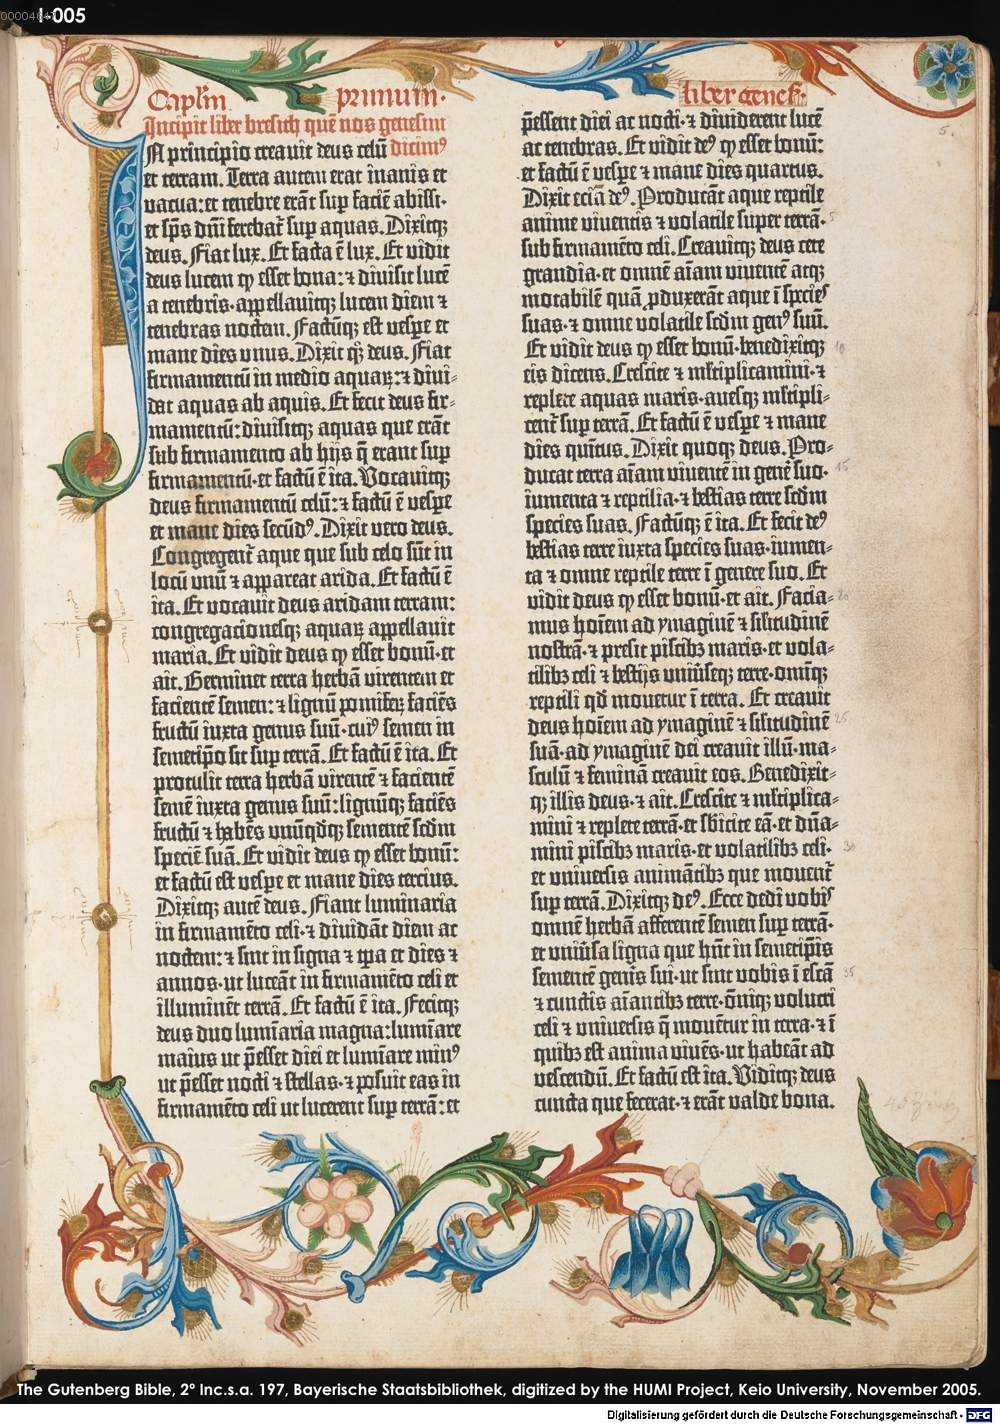
\includegraphics[width=1000px]{images/gutenberg_bible_1x}}
}
\end{center}
\vspace{-1em}
\hfill\footnotesize{Source: Bayerische Staatsbibliothek 
\href{http://daten.digitale-sammlungen.de/bsb00004647/image_13}{(link)}.}
\end{frame}

%--------------------------------------------------------------------
%--- Manual Typesetting
%--------------------------------------------------------------------

\begin{frame}
\frametitle{Manual Typesetting}
\begin{columns}[b]
\begin{column}{0.65\textwidth}
\fbox{%
\adjustbox{trim={1.8cm} {10.3cm} {2.6cm} {2cm}, clip, scale=0.7}{%
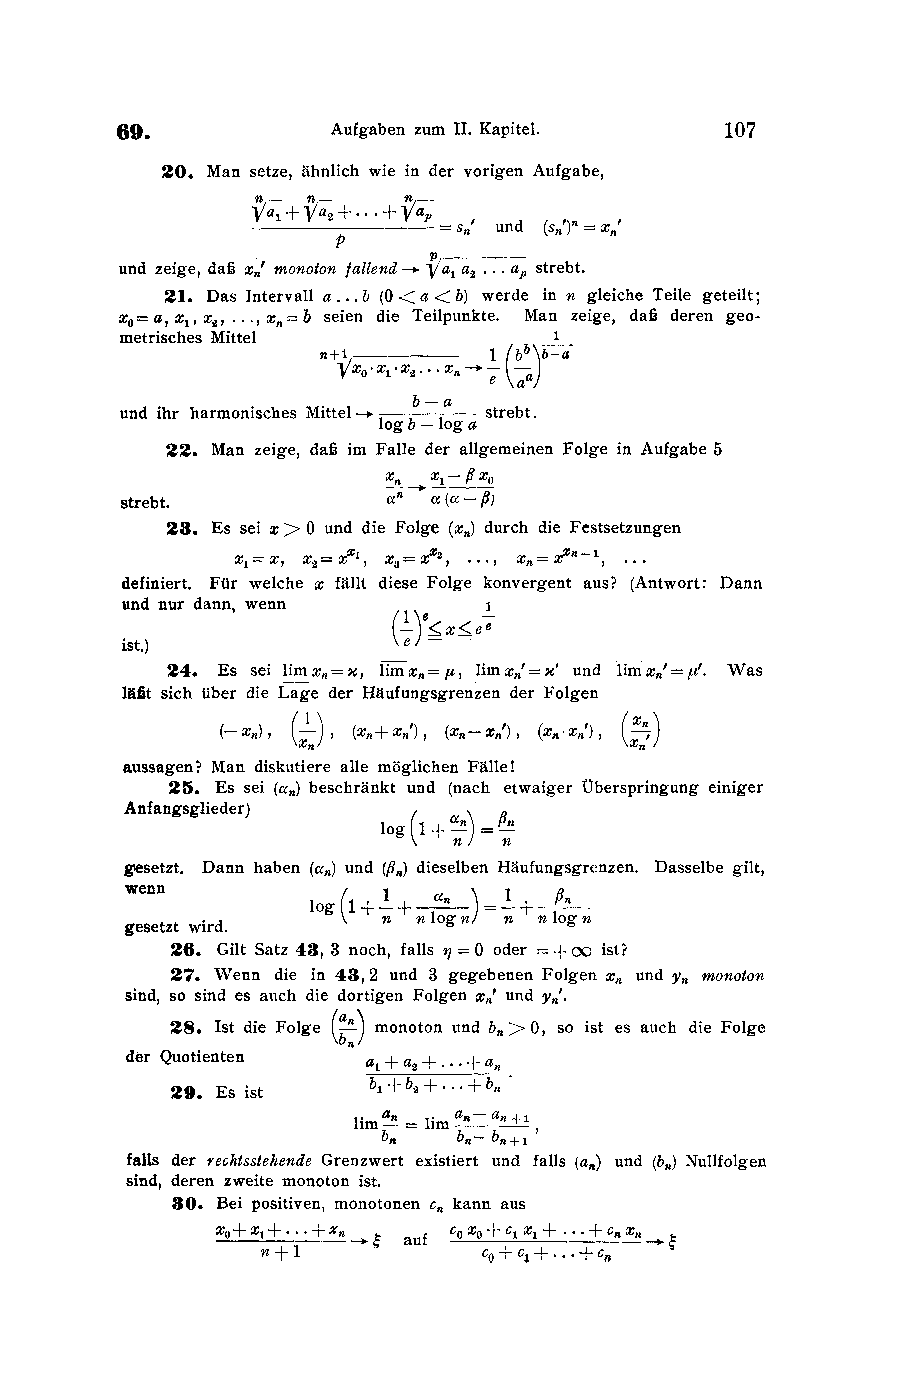
\includegraphics[width=155mm]{images/knopp_reihen_p108}}
}
\end{column}
\begin{column}{0.35\textwidth}
\textsmaller{
Konrad Knopp. \emph{Theorie und Anwendung der Unendlichen Reihen}. Zweite Auflage. Springer. 1924.}
\end{column}
\end{columns}

\end{frame}


%--------------------------------------------------------------------
%--- Written with a Typewriter
%--------------------------------------------------------------------

\begin{frame}
\frametitle{Written with a Typewriter}
\begin{columns}[b]
\begin{column}{0.6\textwidth}
\fbox{%
\adjustbox{trim={1.5cm} {3cm} {1.3cm} {6.5cm}, clip, scale=0.6}{%
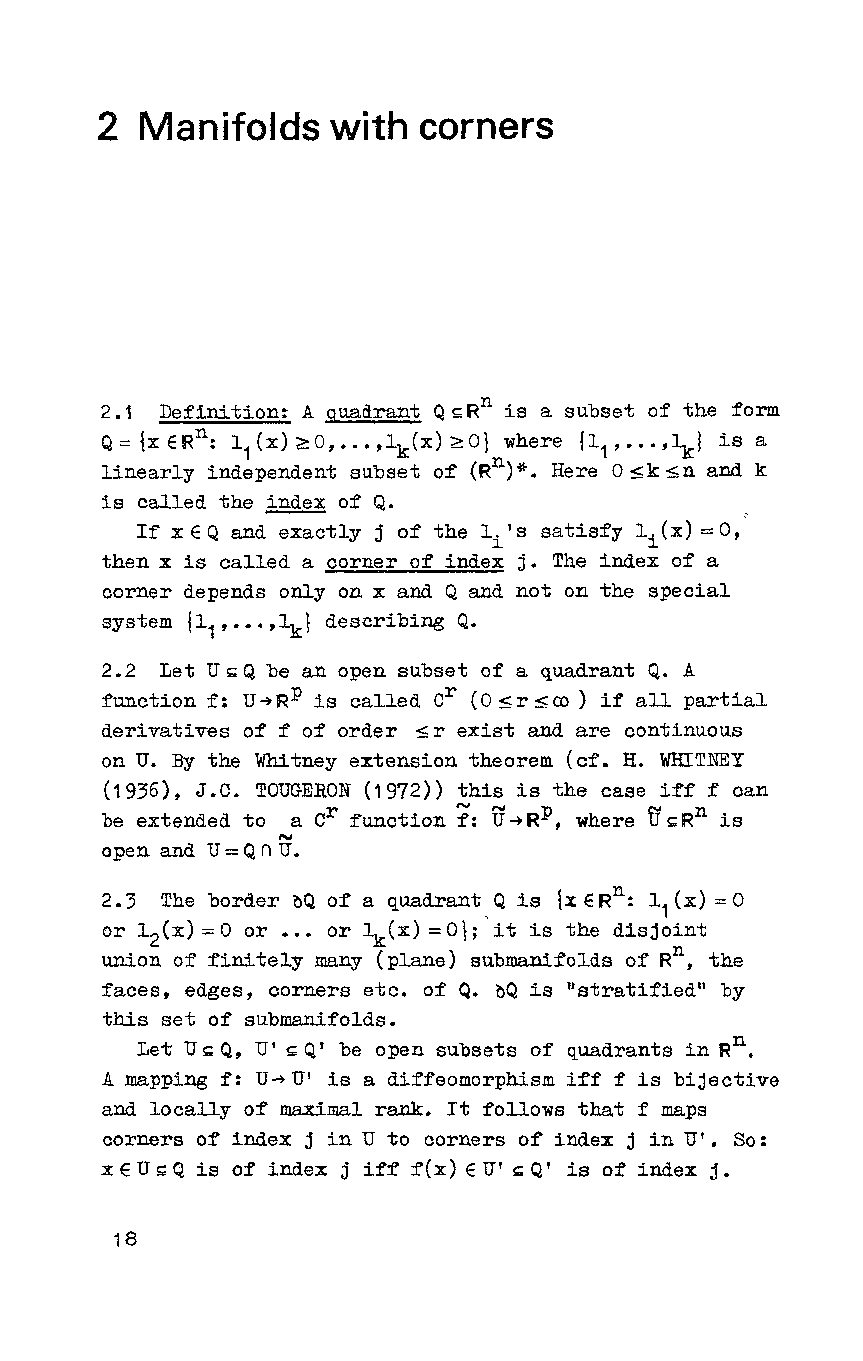
\includegraphics[width=146mm]{images/michor_shiva_p25}}
}
\end{column}
\begin{column}{0.4\textwidth}
\textsmaller{
Peter Michor. \emph{Manifolds of Differentiable Mappings}. Shiva Publishing Limited, Orpington. 1980.}
\end{column}
\end{columns}
\end{frame}

%--------------------------------------------------------------------
%--- Written by Hand
%--------------------------------------------------------------------

\begin{frame}
\frametitle{Written by Hand}
\begin{columns}[b]
\begin{column}{0.57\textwidth}
\fbox{%
\adjustbox{trim={2cm} {7.5cm} {3cm} {2.3cm}, clip, scale=0.6}{%
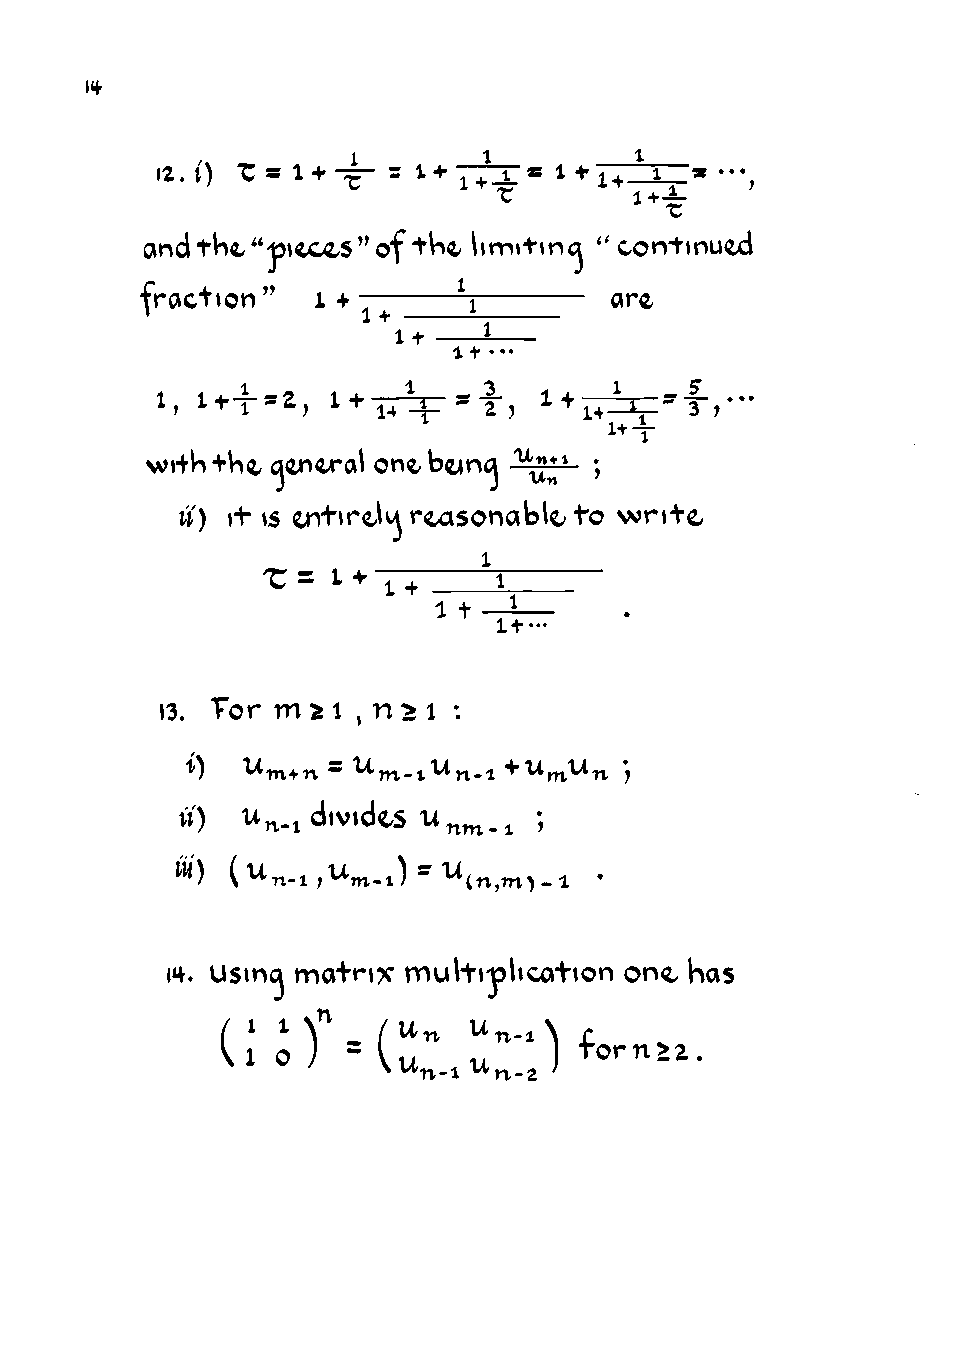
\includegraphics[width=162mm]{images/roberts_number_theory_p29}}
}
\end{column}
\begin{column}{0.43\textwidth}
\textsmaller{
Joe Roberts. \emph{Elementary Number Theory. A Problem Oriented Approach}. The MIT Press, Cambridge. 1977.}
\end{column}
\end{columns}
\end{frame}

%%% Local Variables:
%%% TeX-master: "talk"
%%% End:
